\documentclass{article}
\usepackage[margin=1in]{geometry}
\usepackage{amsmath}
\usepackage{amssymb}
\usepackage{amsthm}
\usepackage{bm}
\usepackage{hyperref}
\usepackage{graphicx}
\usepackage{caption}
\usepackage{listings}
\usepackage{xcolor}
\usepackage{float}
\usepackage{booktabs}
\usepackage{longtable}
\usepackage{multirow}
\usepackage{placeins}
\graphicspath{{figures/}}

% Code style
\lstdefinestyle{code}{
  basicstyle=\ttfamily\small,
  numbers=left,
  numberstyle=\tiny,
  numbersep=8pt,
  keywordstyle=\color{blue},
  commentstyle=\color{teal!70!black},
  stringstyle=\color{orange!70!black},
  showstringspaces=false,
  breaklines=true,
  frame=single,
  framerule=0.3pt,
  rulecolor=\color{black!15}
}
\lstset{style=code}

\title{Toward Autonomous Intelligence: World Models, Continual Learning, and Scientific Frontiers}
\author{}
\date{\today}

\begin{document}
\maketitle

\section{World Models and Memory-Augmented LMs}
\subsection{Integrated architecture}
World models expose latent dynamics of an environment, while memory-augmented language models retain episodic and semantic knowledge. Figure~\ref{fig:world_model_pipeline_en} shows the typical pipeline: sensory streams become latent world states, memories consolidate experiences, and a policy/LLM module plans or converses based on both.
\begin{figure}[H]
  \centering
  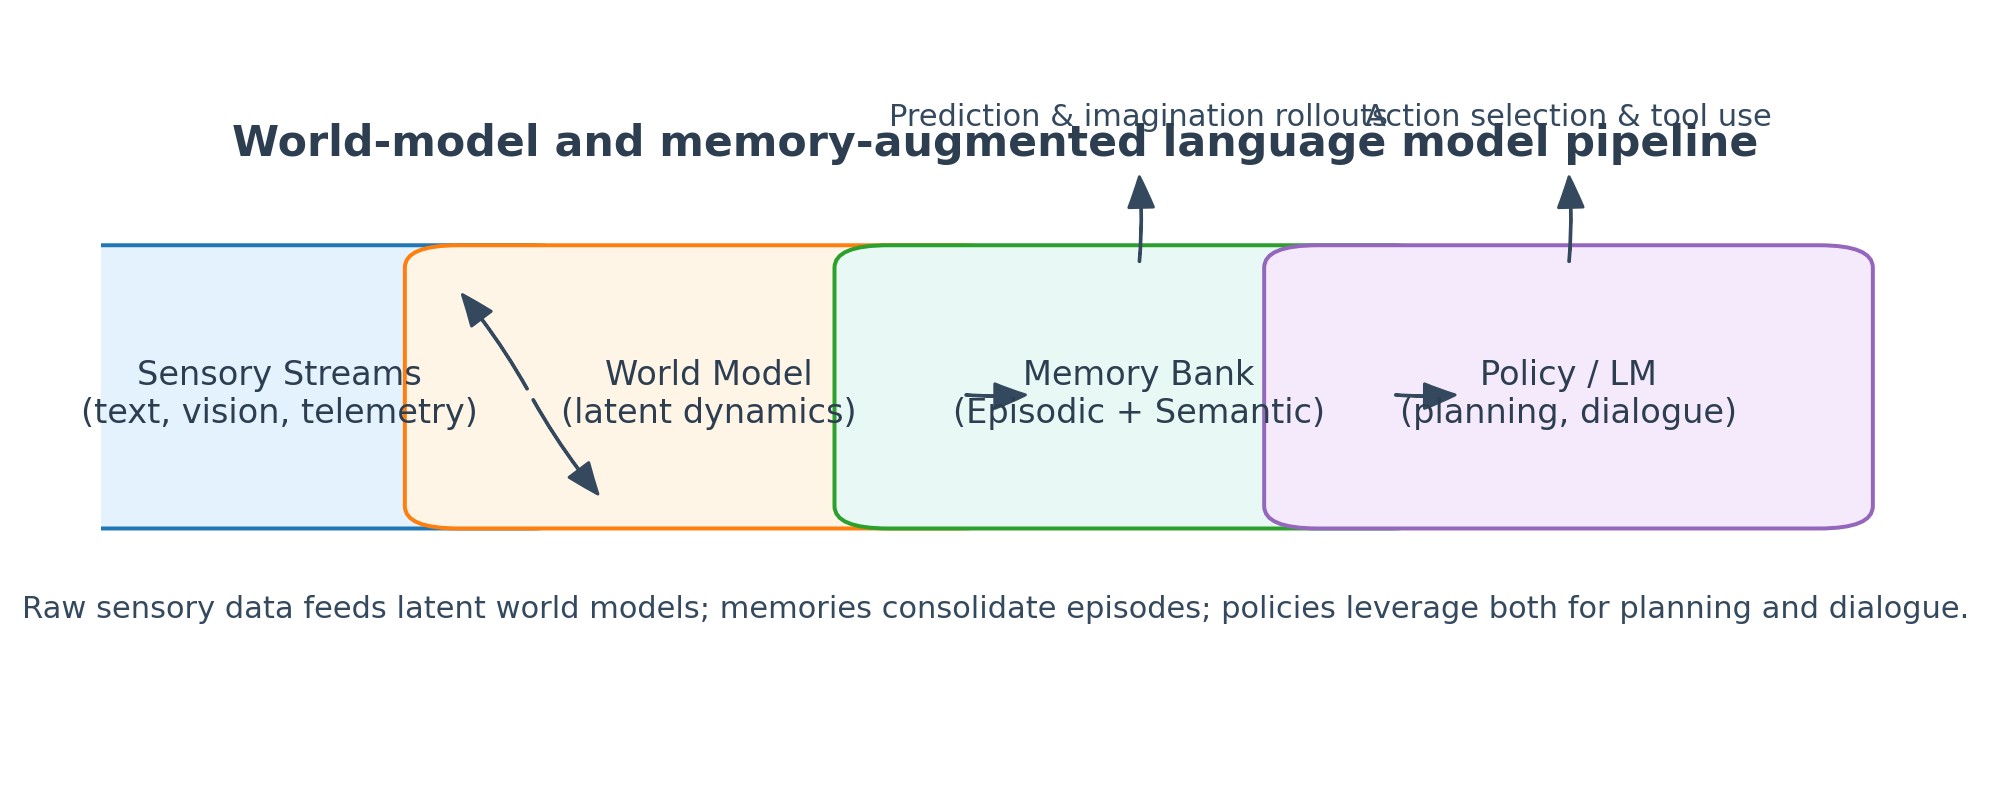
\includegraphics[width=0.95\textwidth]{world_model_pipeline.png}
  \caption{World-model + memory-augmented pipeline feeding policies and language behaviour.}
  \label{fig:world_model_pipeline_en}
\end{figure}

\subsection{Core ingredients}
\begin{itemize}
  \item \textbf{Latent dynamics:} Variational models and transformer state-space models (Dreamer, PlaNet, TD-MPC) learn compact representations.
  \item \textbf{Imagination rollouts:} Generative rollouts simulate future trajectories to evaluate long-horizon outcomes.
  \item \textbf{Model-environment alignment:} Mixed training with real interaction and model-generated data prevents distributional drift.
\end{itemize}

\subsection{Memory augmentation}
\begin{itemize}
  \item \textbf{Working memory:} On-the-fly context buffers, KV caches, scratchpads for current tasks.
  \item \textbf{Episodic memory:} Vector databases or logs storing past experiences for retrieval-augmented reasoning.
  \item \textbf{Semantic memory:} Curated knowledge bases, skill graphs, and workflows enabling transfer across tasks.
  \item \textbf{Memory hygiene:} Write policies, forgetting mechanisms, deduplication, and conflict resolution keep memory reliable.
\end{itemize}

\section{Self-Improving and Continual Learning}
\subsection{Self-improvement loop}
\begin{enumerate}
  \item \textbf{Self-observation:} Capture reasoning traces, tool usage, user feedback, and failure examples.
  \item \textbf{Self-diagnosis:} Auxiliary evaluators classify errors (logic, safety, alignment).
  \item \textbf{Self-update:} Apply replay and gradient updates via online tuning, LoRA, or EMA weight averaging.
  \item \textbf{Verification:} Run offline/online tests, stage rollout, and keep rollback paths ready.
  \item \textbf{Governance:} Log every change, maintain audit trails, and align updates with policy constraints.
\end{enumerate}

\subsection{Continual learning toolbox}
\begin{itemize}
  \item \textbf{Regularization-based:} EWC, MAS, SI penalize parameter drift on important directions.
  \item \textbf{Replay-based:} Store representative samples or generate synthetic ones (generative replay, distillation buffers).
  \item \textbf{Modular updates:} Adapter stacks, expert routers, or progressive networks isolate new skills.
  \item \textbf{Task detection:} Distribution shift monitoring, uncertainty estimation, and novelty detection trigger adaptation.
\end{itemize}

\subsection{Evaluation metrics}
\begin{itemize}
  \item Average accuracy over all tasks and learning stages.
  \item Forgetting index (gap between original and current performance).
  \item Sample efficiency, compute, and energy per task.
  \item Stability-plasticity balance: trade-off between retaining old skills and learning new ones.
\end{itemize}

\section{Agentic Systems (MetaGPT, Voyager)}
\subsection{Ecosystem overview}
Figure~\ref{fig:agentic_ecosystem_en} summarizes the agentic ecosystem: MetaGPT orchestrates role-based teams, Voyager learns in open worlds, continual learning pipelines update knowledge, and scientific applications close the deployment loop.
\begin{figure}[H]
  \centering
  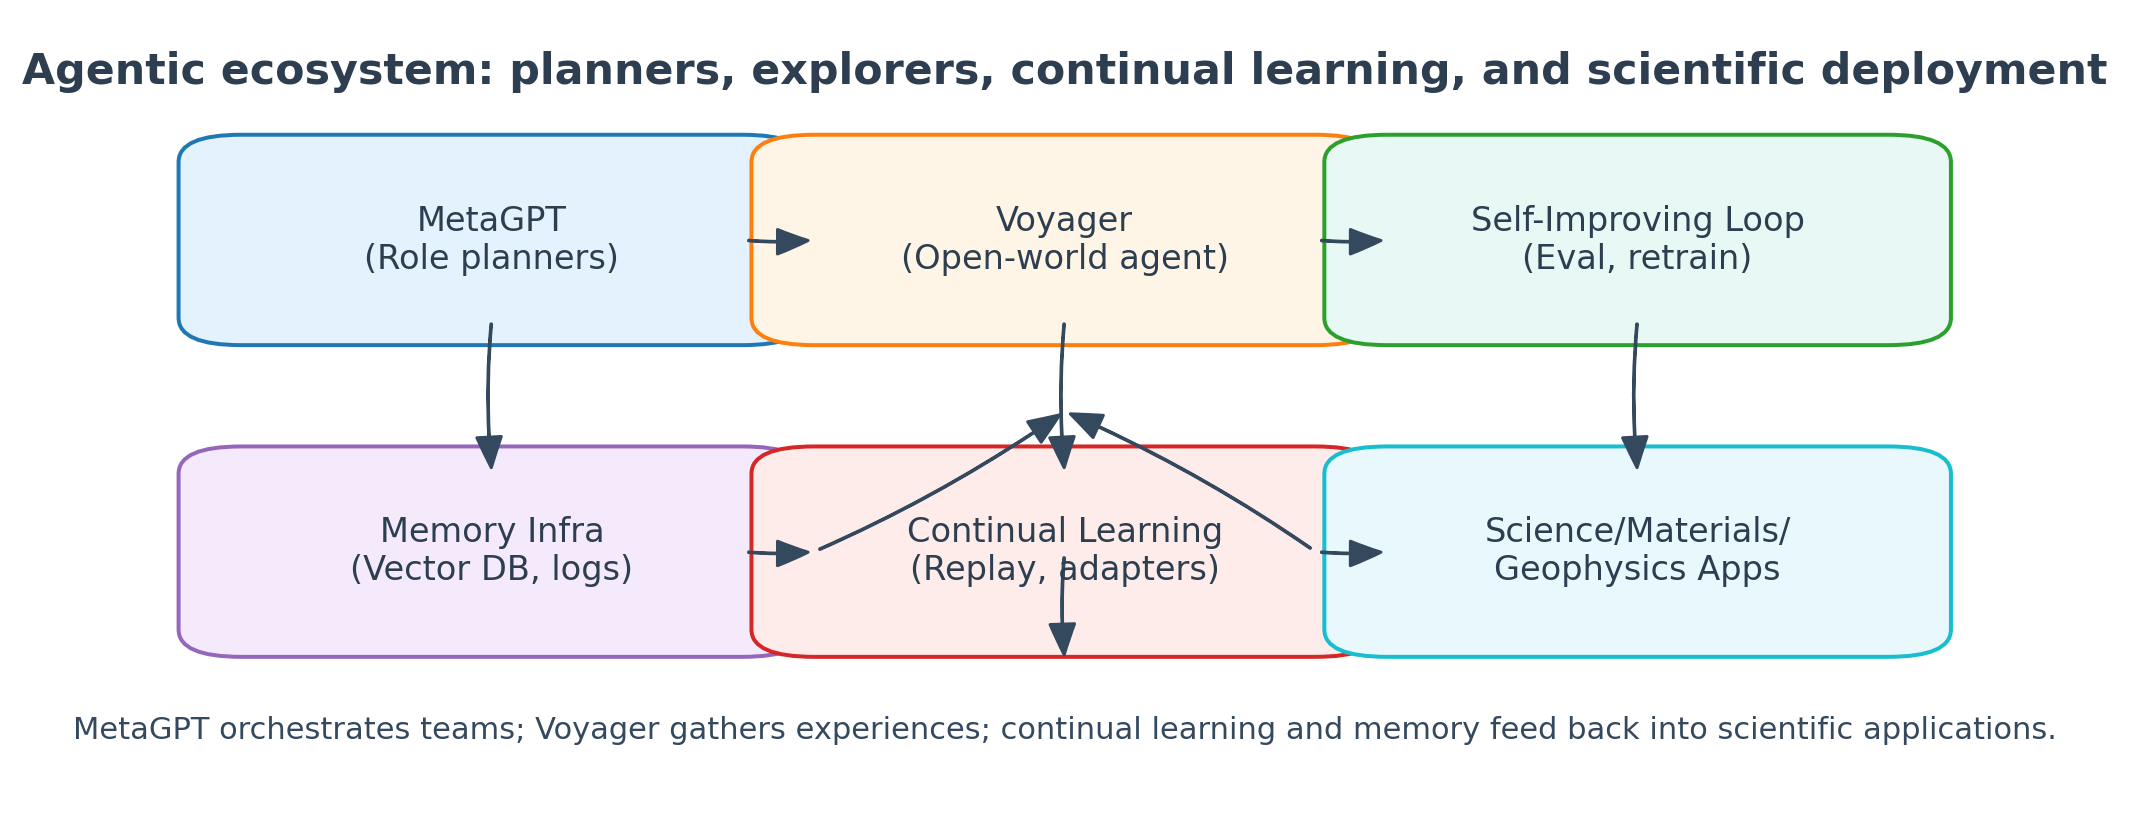
\includegraphics[width=0.95\textwidth]{agentic_ecosystem.png}
  \caption{Agentic ecosystem linking planners, explorers, continual learning, and scientific deployments.}
  \label{fig:agentic_ecosystem_en}
\end{figure}

\subsection{MetaGPT}
\begin{itemize}
  \item \textbf{Role orchestration:} Encodes software roles (PM, architect, engineer, QA) with custom prompts and memory slots.
  \item \textbf{Pipeline automation:} Requirement parsing, design docs, code generation, testing, and review happen in sequence.
  \item \textbf{Shared memory:} Task boards, knowledge bases, and artifact stores keep agents aligned.
  \item \textbf{Use cases:} Software engineering, content creation, data analysis, cross-functional workflows.
\end{itemize}

\subsection{Voyager}
\begin{itemize}
  \item \textbf{Open-ended exploration:} Autonomous discovery of tools, recipes, and strategies in Minecraft-like environments.
  \item \textbf{Skill library:} Stashes successful scripts and subroutines in a searchable repository.
  \item \textbf{Self-improvement:} Learns from failures, revises prompts, and rewrites code via introspective critique.
  \item \textbf{Extensions:} Robotics, simulation control, and integration with world models plus planners.
\end{itemize}

\subsection{Design principles}
\begin{itemize}
  \item Role-based governance and capability segregation.
  \item Hierarchical memory (episodic, semantic, tool) with fast retrieval.
  \item Modular self-improvement loops with pluggable evaluators.
  \item Safety: audit trails, rate limits, human-in-the-loop oversight.
\end{itemize}

\section{AI for Science, Materials, and Geophysics}
\subsection{Autonomous scientific discovery}
\begin{itemize}
  \item \textbf{Research automation:} Literature mining, hypothesis generation, experiment scripting, and results synthesis.
  \item \textbf{Robotic labs:} Closed-loop execution with autonomous instruments and feedback to LLM planners.
  \item \textbf{Data stewardship:} Unified repositories for lab notebooks, sensor data, simulation outputs, and knowledge graphs.
\end{itemize}

\subsection{Materials design}
\begin{itemize}
  \item \textbf{Generative design:} World models predict property landscapes; Bayesian optimization selects promising candidates.
  \item \textbf{Multiscale modeling:} Integrate molecular dynamics, quantum chemistry, and continuum simulations via shared memory.
  \item \textbf{Closed-loop experimentation:} Iterate design-synthesize-characterize-analyze cycles autonomously.
\end{itemize}

\subsection{Geophysics and energy}
\begin{itemize}
  \item \textbf{Inverse modeling:} Fuse seismic, EM, and remote sensing data for precise subsurface reconstructions.
  \item \textbf{Hazard assessment:} Detect anomalies, forecast earthquakes or landslides, and propose mitigation strategies.
  \item \textbf{Carbon management:} Optimize monitoring of carbon capture and storage, simulate reservoir evolution.
\end{itemize}

\subsection{Challenges and outlook}
\begin{itemize}
  \item Secure data sharing and privacy-preserving collaboration across institutions.
  \item Multimodal fusion with strong physical priors and uncertainty quantification.
  \item Human-AI co-development: ensuring interpretability, controllability, and accountability.
  \item Ethical governance: auditing decisions, fail-safe mechanisms, and regulatory compliance.
\end{itemize}

\section*{Operational recommendations}
\begin{itemize}
  \item Modularize world models, memory layers, evaluators, and agent controllers for rapid iteration.
  \item Instrument self-improvement pipelines: data validation, simulation, human review, deployment gating.
  \item Introduce safety checks and red-teaming for agentic systems; maintain human-in-the-loop controls.
  \item Collaborate with domain scientists to build shared benchmarks, simulators, and experimental platforms.
\end{itemize}

\section*{Further reading}
\begin{itemize}
  \item Ha and Schmidhuber. ``World Models.'' NeurIPS, 2018.
  \item Hafner et al. ``Mastering Diverse Domains via World Models (DreamerV3).'' arXiv, 2023.
  \item Hong et al. ``MetaGPT: Meta Programming for Multi-Agent Collaborative Framework.'' arXiv, 2023.
  \item Wang et al. ``Voyager: An Open-Ended Embodied Agent with LLMs.'' arXiv, 2023.
  \item AI4Science Community. ``Autonomous Discovery in Materials and Chemistry.'' Nature, 2024.
\end{itemize}

\end{document}

